\section{ Diskrétní obraz, jeho vlastnosti a reprezentace (model kamery, projekce, digitalizace, metriky), binární, šedotónový a
barevný obraz - barevné formáty, souborové formáty.}
Informace jsou z přednášky 2 diskretní obraz: $http://vision.uamt.feec.vutbr.cz/ZVS/lectures/03_Diskretni_obraz.pdf$
\subsection{Digitální obraz}

Diskretní obraz je matematickou reprezentací vzorkovaného skutečného obrazu. Obraz je reprezentován maticí s rozměry MxN, kde M je šířka a N 
výška zachyceného obrazu. Dále diskrétní obraz uchovává dimenzi. Když je obraz 1 dimenzionální tak se jedná o obraz stupni šedi. Pokud 
je 3 dimenzionální tak se jedná o barevný obraz (3 dimenze - RGB (red,green, blue)).
 \begin{figure}[h!]
 \vspace{-5mm}
 \centering
 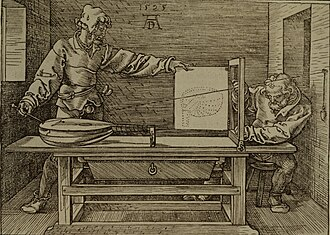
\includegraphics[width=0.7\textwidth]{img/obr1.jpg}
 \caption{Dürer - Man Drawing a Lute}
 \vspace{-5mm}
 \end{figure}
%jestli chcete obrázek tak si to odkomentujte
\subsection{Projekce}
jev kdy zachycujeme 3D obraz na 2D snímač, ztrácíme informace o jedné dimenzi. 

\subsection{Model kamery}
Camera obscura (temná komora) - jedná se o tmavou komoru do které vstupuje světlo pouze jedním bodem (v angličtině pinhole). 
využívá perspektivní projekci (napodobuje lidské oko, kde střed promítání je střed čočky, na senzor následně dopadají paprsky převráceně
, za následek vzdálené objekty jsou menší než ty blíže). Matematický popis celé kamery je na principu podobnosti trojúhelníků. První 
trojúhelník vzniká pata objektu - vrchol objektu a vstupní bod do komory, druhý vzniká pata obrazu(senzoru) vrchol obrazu a dírka. 
 \begin{figure}[h!]
 \vspace{-5mm}
 \centering
 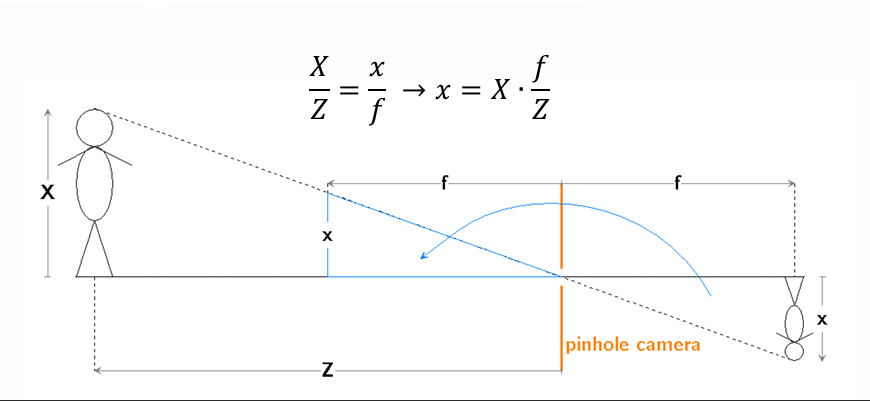
\includegraphics[width=0.7\textwidth]{img/troj.png}
 \caption{perspektivní projekce}
 \vspace{-5mm}
 \end{figure}
\subsection{Digitalizace}
Převod analogového signálu na diskretní. Dva duležité pojmy: Vzorkování - určuje rozlišení obrazu(digitalizace signálu v čase), kvantování
- udává počet úrovní (hloubku signálu, je to digitalizace signálu v amplitudě). Při pořízení snímku dochází nejdříve k primárnímu Vzorkování-
dochází automaticky při zachycení světla na maticový snímač, buňky snímače můžou mít různé tvary ale jsou nejčastěji ortogonální (čtvercové)
. U analogových snímačů k primárnímu vzorkování nedochází. - Následně probíhá softwarové(sekundární) vzorkování, dochází k snižení/zvýšení 
rozlišení, interpolaci(lineární, kubická, nejbližší soused) a filtraci (Hermit, Lanczos..). Kvantování probíhá pomocí A/D převodníku, podle 
počtu bitů N, je následně $2^N$ úrovní. Kamery mívají 12 nebo 16 bitů. Využívá se 8.(často, může i více)

\subsection{Reprezentace}
Obraz je reprezentován zapomocí matice obrazových bodů. To je vyjádřeno pomocí obrazové funkce kde g(x,y) ~ statický obrat a g(x,y,t) ~
dynamický obraz(sekvence snímků). Obrazová funkce je buď to reprezentována zapomocí skaláru - pak se jedná o šedotónový obraz. 
Nebo zapomocí vektoru - pak se nejčastěji jedná o RGB. g -vyjadřuje obrazovou funkci(jas u obrazu, teplota u termovize atd.). 
\subsection{Metrika}
Vyjadřuje odlehlost (vzdálenost 2 bodů v prostoru/rovině/přímce), vzdálenost je definovaná pro konečnou dimenzi, je značená pomocí "ro"
a platí axiomi:   1. Nezápornost 2. totožnost 3. symetrie 4. trojuhelnikova nerovnost. V ortogonálním ratru jsou použitelné metriky na základě
Minkowského vzdálenosti. Typický příklad: euklidovská vzdálenost, manhattanská vzdálenost a šachovnicová. 

\subsection{Druhy obrazu}
Binární - obsahuje pouze 0 a 1, výhodné na uchovávání, zabere pouze místo matice MxN.
Monochromatický(šedotónový) - uchovává stupně šedí, nejčastěji obsahuje 255 úrovní. Pro uchovávání je potřebné MxNxpočet bitů.
Multichromatický(barevný) - obsahuje $n*2^k$ úrovní, často n = 3 a k = 8. Pro uchovávání je nutné NxM*n*k.





\section{ Konvoluční integrál, korelace obrazových signálů, okolí bodu, lineární a nelineární filtry (masky - detekce hran a rohů,
filtrace šumu), typy šumu.}

Note: píšu pouze s jednou rukou, pomohl jsem si s gemini, informace jsem si kontroloval. Mělo by to sedět.
 \begin{figure}[h!]
 \vspace{-5mm}
 \centering
 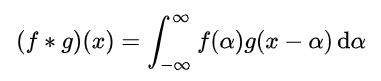
\includegraphics[width=1\textwidth]{img/konv.png}
 \caption{Konvoluční integrál}
 \vspace{-5mm}
 \end{figure}

\subsection{Konvoluce vs Korelace}
Konvoluce vs. Korelace v moderní praxiV současném digitálním zpracování signálů a hlubokém učení se rozdíl mezi konvolucí a korelací často stírá. 
Většina knihoven pro konvoluční neuronové sítě (CNN), jako je TensorFlow nebo PyTorch, ve skutečnosti pod kapotou implementuje křížovou korelaci, i když se operace nazývá 
konvoluce.Hlavní technické rozdíly:Otočení filtru (Kernel Flipping): Jediný matematický rozdíl spočívá v tom, že u čisté konvoluce je nutné jádro (filtr) otočit o 180 stupňů.
Korelace pracuje s maskou v jejím původním stavu. U neuronových sítí je toto otočení nepodstatné, protože síť se váhy v jádru učí sama – pokud potřebuje "otočený" filtr k 
rozpoznání příznaku, prostě si ho tak natrénuje.Matematické vlastnosti: Konvoluce je z čistě matematického hlediska výhodnější, protože splňuje důležité zákony, které usnadňují
komplexní výpočty:Komutativita: $a * b = b * a$ (nezáleží na pořadí operace).Asociativita: $(a * b) * c = a * (b * c)$ (umožňuje seskupování operací).
Distributivita: $a * (b + c) = (a * b) + (a * c)$.Funkční význam: * Konvoluce zkoumá vliv systému na signál. Popisuje, jak se vstupní data mění při průchodu určitým 
prostředím nebo filtrem.Korelace zkoumá shodu (podobu). Porovnává vstupní data s maskou (šablonou) a hledá místa, kde se tyto dva vzory nejvíce překrývají.
\subsection{typy šumů}
Šum - data bez významu, jsou vedlejším efektem ostatních aktivit(kvantizace, nestabilita snímače, atd..)

Pepper and salt - impulsní šum projevující se zrněním, u obrazu s více jasovými úrovněmi.
Gaussovský -  hustota pravděpodobnosti šumu má gaussovo rozložení.
Poissonovský (Photon counting) – u senzorů pracujících jako čítač fotonů (CCD)
bílý = idealizovaný, používá se pro simulace nejhorších degradací obrazu, ve výkonovém spektru má rovnoměrně zastoupeny všechny frekvence
kvantizační = není použit dostatečný počet jasových úrovní
aditivní = vzniká při přenosu obrazu nebo snímání 
multiplikativní = šum TV rasteru, charakter vodorovných pruhů

\subsection{lineární a nelineární filtry}
Lokální lineární filtry
intenzita bodu je rovna součtu součinů intenzit bodů v okolí a příslušných váhových 
koeficientů (matice koeficientů = filtr). Lokální nelineární filtry- intenzita bodu není dána lineární kombinací vstupních hodnot, ale jiným algoritmem, 
nejčastěji vybírá některou z hodnot ve stanoveném okolí.
Mezi lineární filtry řadíme průměrovací a s gaussovým rozložením. Do nelineárních spadá Medián(Kvantil - vybere z kernelu střední hodnotu. Nerozmazává hrany, ale ztrácíme detaily)
, Modus (hodnota, která se v okolí vyskytuje nejčastěji - nejčetnější hodnota intenzity), Min/Max(eroze/dilatace- min - potlačí šum v tmavých oblastech a zmenšuje čáry a eroze objektu, 
max naopak potlačí šum ve světlých oblastech, ale zesiluje čáry a zvětšuje objekt), konzervativní(k odfiltrování izolovaných pixelů s velmi nízkou/vysoko intenzitou -např. sůl a pepř
-najde v kernelu min a max, pokud hodnota je v tomto intervalu zůstane ponechána. jinak je nahrazen novou hodnotou odvozenou z okolí - třeba minimem z okolí pokud byla hodnota nižší),
rotující maska(V tomto případě je zvolená maska rotována kolem filtrovaného bodu, např. jako na následujícícm obrázku pro masku 3×3, kdy je celkem devět možných poloh masky. Pro každou 
její pozici je spočítána míra homogenity jako např. součet diferencí. Filtrace se pak provádí jen pro jednu polohu masky, pro níž je míra homogenity nejvyšší 
(nejnižší diference/rozptyl). Takto je nalezeno to okolí bodu, které k němu patří s největší pravděpodobností. Filtrace rotující maskou tedy částečně řeší problémy s 
rozmazáváním a porušováním tenkých čar a ostrých rohů, nevýhodou je však vyšší časová náročnost výpočtu.)
 \begin{figure}[h!]
 \vspace{-5mm}
 \centering
 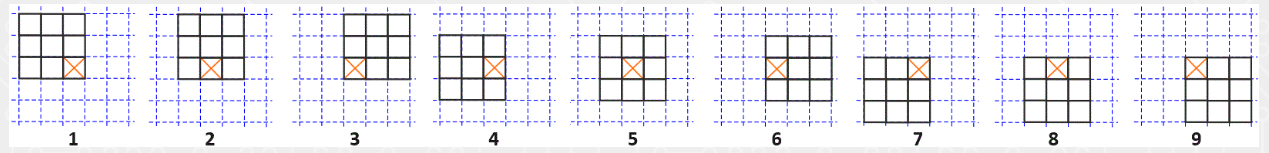
\includegraphics[width=1\textwidth]{img/rotmaska.png}
 \caption{Rotující maska}
 \vspace{-5mm}
 \end{figure}

 \subsection{Okolí bodu}
 1D-množina složená z aktualního bodu a jeho sousedů ve vzdálenosti. 2D- 4 okolí -body sousedící hranou(ortogonální směry NESW), 8 mi okolí-body sousedící hranou nebo rohem,
 6 okolí - body sousedící hranou v hexagonálním rastru.

 \subsection{Detekce hran a rohů}
\begin{itemize}
    \item Hrany, čáry a body jsou nositeli informací o různých oblastech v obrazu, zejména pak o hranicích objektů[cite: 25].
    \item Hrana je definována jako místo v obrazu, kde dochází ke strmé změně obrazové funkce $f(x,y)$[cite: 27].
    \item Strmost obrazové funkce určuje velikost (magnitudu) hrany, normála gradientu pak její směr[cite: 28].
    \item Rozdíl spočívá v tom, že hrana je chápána jako hranice mezi dvěma oblastmi, zatímco čára nebo bod je lokální změna jasové funkce v jinak homogenní oblasti[cite: 29, 30].
\end{itemize} 
\begin{itemize}
    \item Protože je obrazová funkce $f(x,y)$ dvourozměrná, její gradient je vektor[cite: 46]: 
    \begin{equation}
        \nabla f(x,y) = \begin{bmatrix} G_x \\ G_y \end{bmatrix} = \begin{bmatrix} \frac{\partial f(x,y)}{\partial x} \\ \frac{\partial f(x,y)}{\partial y} \end{bmatrix}
    \end{equation} [cite: 47]
    \item Pro diskrétní obraz jsou složky vektoru gradientu aproximovány diferencemi: $G_x \approx \Delta_x f(x,y) = f(x,y) - f(x-n, y)$[cite: 70, 71].
    \item \textbf{Velikost gradientu (G):} Lze aproximovat euklidovskou vzdáleností ($\sqrt{\Delta_x^2 f(x,y) + \Delta_y^2 f(x,y)}$) [cite: 76], součtem absolutních hodnot ($|\Delta_x f(x,y)| + |\Delta_y f(x,y)|$) [cite: 74], nebo maximem ($\max\{|\Delta_x f(x,y)|, |\Delta_y f(x,y)|\}$)[cite: 95].
    \item \textbf{Směr gradientu ($\theta$):} $\theta(x,y) = \arg(\Delta_x f(x,y), \Delta_y f(x,y))$[cite: 103]. Úhel je měřen vzhledem k ose x[cite: 68].
\end{itemize}
\begin{itemize}
    \item Výpočet diferencí lze zapsat jako maticové operátory[cite: 109]. Detekci hran pak lze realizovat konvolucí:
    \begin{equation}
        g(x,y) = f(x,y) * h
    \end{equation}
    kde $h$ je maska operátoru[cite: 115, 116].
    \item Zvýraznění vyšších prostorových frekvencí v obrazu s sebou nese nevýhodu: kromě skutečných hran je zvýrazněn také šum[cite: 128].
\end{itemize}
Aproximují první derivaci obrazové funkce[cite: 142]. Tyto operátory většinou nejsou invariantní vůči rotaci[cite: 148].
\begin{itemize}
    \item \textbf{Robertsův kříž (1963):} Jednoduchý a výpočetně nenáročný operátor[cite: 151]. Oproti ostatním operátorům je hodně citlivý na šum kvůli malému počtu zpracovaných pixelů[cite: 152].
    \item \textbf{Prewittové operátor (1966):} Využívá symetrický kernel v obvyklém rozměru $3 \times 3$[cite: 163].
    \item \textbf{Sobelův operátor (1968):} Stejný mechanismus jako operátor Prewittové[cite: 183]. Rozdíl je pouze ve váze koeficientů u sousedů ve čtyř-okolí vzhledem ke směru detekce[cite: 184].
    \item \textbf{Kirschův a Robinsonův operátor:} Nesymetrický kernel v obvyklém rozměru $3 \times 3$[cite: 201, 209]. Kombinuje různý počet koeficientů s různými hodnotami[cite: 202, 211].
\end{itemize}
Je výpočetně jednodušší a přesnější hledat inflexní body hran, tedy průchody nulou druhé derivace (tzv. zero-cross operátory)[cite: 286, 294, 295]. Tyto operátory jsou nativně invariantní vůči rotaci[cite: 296].
\begin{itemize}
    \item \textbf{Laplaceův operátor:} Pro aproximaci výpočtu druhé derivace se výhradně používá Laplacián[cite: 298]. Má stejné vlastnosti ve všech směrech, tj. je izotropický[cite: 300].
    \item \textbf{LoG operátor (Laplacian of Gaussian):} Aplikace Laplaciánu po filtraci obrazu Gaussovým filtrem[cite: 303]. Derivace Gaussova filtru jsou vypočítány předem, tj. nezávisí na obrazových datech[cite: 305].
\end{itemize}
\begin{itemize}
    \item Úprava obrazu s charakterem horní propusti, která zvyšuje podíl složek o vyšších frekvencích (zvýrazňuje hrany)[cite: 309].
    \item Realizováno odečtením váženého obrazu hran od vstupního obrazu:
    \begin{equation}
        g(x,y) = f(x,y) - c \cdot S(x,y)
    \end{equation}
    kde $c$ určuje míru ostření a $S(x,y)$ je obraz hran[cite: 310, 311, 312].
    \item Odečtením vysokých frekvencí se prohlubují extrémy[cite: 314]. Pro výpočet strmosti se nejčastěji používá Laplaceův operátor[cite: 317].
\end{itemize}
    
\section{Jasové transformace (histogram, kumulovaný histogram - ekvalizace, jasové korekce), geometrické transformace
(aproximace, bilineární a afinní transformace, homogenní souřadnice, interpolace souřadnic, korekce zkreslení, rotace /
měřítko).}
\subsection{Jasové transoformace}
Změna hodnot jasu, podle určité funkce. Vstupem i výstupem je obraz stejných parametrů(rozlišení, bitová hloubka). 
Neslouží k rozpoznávání ani identifikaci objektů. Většinou součást předzpracování obrazu(úprava kontrastu, zvýšení jasu). 
Dělení jasových transformací:
\begin{itemize}
    \item Globální - hodnota pixelu je vypočítána na základě celého obrazu, značeno symbolem $\Omega(I) \xrightarrow{T} f(x, y), \quad \forall x, y \in \Omega(I)$. Mezi Globální
    transformace patří Integrální obraz, Fourierova transformace. 
    \item Lokální - hodnota je vypočítána na základě lokálního okolí. $\Omega(x,y) \xrightarrow{T} f(x, y), \quad \forall x, y \in \Omega(I)$. Patří sem redukce šumu, vyhlazování
    obrazů, zvýraznění rysů(hrany).  K vyhlazování obrazu lze využít:
    \begin{itemize}
        \item prostý/vážený průměr - Řeší se konvolucí(*), výsledek je ovlivněn velikostí konvolučního jádra
        \item Medián - Nelze řešit konvolucí, je to pouze aditivní a multiplikativní operace. Ze seřazených hodnot se vybírá prostřední hodnota. Lze vybírat i kvartili atd. Nejen kvantili
        \item Modus  
        \item jiné funkce (min,max)
    \end{itemize}
    \item Bodové - Hodnota je vypočítána na základě téhož pixelu $f'(x, y) \xrightarrow{T} f(x, y), \quad \forall x, y \in \Omega(I)$ - Slouží k jasové korekci(každý pixel korigován 
    samostatně), převodní charakteristika(všechny pixely korigovány stejně), roztažení histogramu.  
\end{itemize}
\subsubsection{Bodová jasová transformace}
Kompenzace systematické chyby při pořizení obrazu(z důvodu: nerovnoměrné osvětlení, rozdílná citlivost prvků snímače,nedokonalá přenosová funkce). Pro korekci je nutné 
určit degradační fci a předpokládat multiplikativní charakter poruchy.
\begin{itemize}
    \item g(x,y) = nekorigovaný obraz
    \item e(x,y) = degradační funkce - modeluje poruchu, existují: Analytický model -aproximace poruchy analytickou plochou,dán obecně nelineární rovnicií určenou z apriorní explicitní
    informace. Empirický - etalonový snímek, pořídí se snímek g(x,y) při explicitně určené scéně g'(x,y), funkce je pak určena podílem g/g'.
    \item f(x,y) = korigovaný obraz 
\end{itemize}
$f(x,y) = e(x,y)*f(x,y)$

Převodní charakteristika - transformace T jasové stupnice g vstupního obrazu na jasovou stupnici f výstupního obraz f = T(g). Implementace pomocí Lute

\subsection{Ekvalizace histogramu} 
= transofrmace jasové stupnice, po níž jsou jasové složky zastoupeny rovnoměrně - pro pozorovatele se to projeví zvýšením kontrastu. Definovaná normalizace pro jasové porovnávání
dvou obrazových segmentů. 

Cíl ekvalizace - Nalézt neklesající transformační funkci t na základě histogramů h (i) vstupního obrazu takovou, aby histogram g (i) výstupního obrazu byl uniformní na celém 
intervalu hodnot jasu.
\textbf{Vstup výpočtu} = histogram vstupního obrazu \\
\textbf{Výstup výpočtu} = výstupní obraz
\[
\sum_{i = p_0}^{p_k} h(i) = \sum_{i = q_0}^{q_k} g(i)
\]
\[
\Rightarrow \text{rozlišení snímku } M \times N \text{ se nemění}
\]
\[
\approx \text{energie histogramů je stejná}
\]
\textbf{Histogram určen vstupním obrazem} \\
$\approx$ libovolné rozložení

\textbf{Ekvalizovaný histogram} \\
$\approx$ uniformní rozložení

\textbf{U diskrétního obrazu je teoretická výška čar:}
\[
n_u = \frac{M \cdot N}{q_k - q_0},
\]
\[
\begin{cases}
M, N = \text{rozměry obrazu} \\
q \in \langle q_0; q_k \rangle = \text{definiční obor histogramu}
\end{cases}
\]
Postup výpočtu ekvalizace : 1) histogram obrazu, 2) kumulovaný histogram 3) normalizace kumulovaného histogramu na převodní charakteristiku 4) transformace jasové stupnice. 

\[
q = \frac{q_k - q_0}{M \cdot N} \cdot h_k(p) + q_0
      = k_1 \cdot h_k(p) + k_2
\]


\begin{figure}[h!]
 \centering
 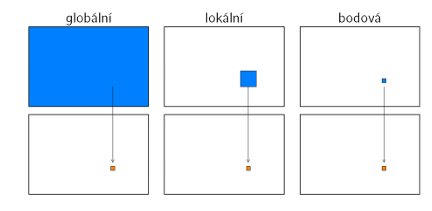
\includegraphics[width=0.8\textwidth]{img/globalni.png}
 \caption{Globalni x Lokalni x Bodova jasová transformace}
 \end{figure}
\subsubsection{Histogram}
    grafické zobrazení četnosti jasové hodnoty. Na ose x jsou jasové úrovně. Např pro uint8 $<0,255>$, na ose Y je vyjádřena četnost této úrovně. 
\begin{figure}[h!]
 \vspace{-5mm}
 \centering
 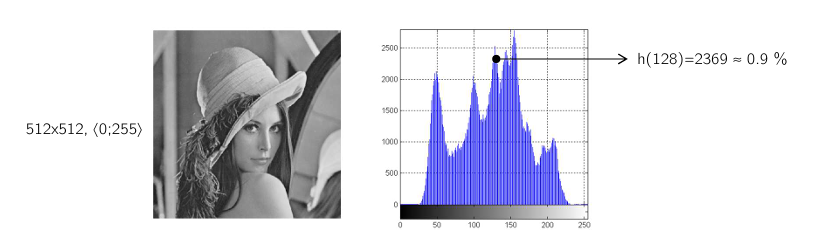
\includegraphics[width=1\textwidth]{img/histogram.png}
 \caption{Histogram Leny}
 \vspace{-5mm}
 \end{figure}

 \subsection{Kumulaticvní histogram}
 Vzniká integrací klasického histogramu podle proměnné $q$. Výsledkem je spojitá neklesající funkce. Normalizovaná verze kumulovaného histogramu se používá jako převodní funkce.
 \begin{equation}
    h_k(q)=\sum_{i = 0}^{q} h(i) = h_k(q-1)+h(q)
 \end{equation}

 \subsection{geometrická transformace}
 Geometrická transformace = transformace souřadnic obrazových bodů a s ní spojená interpolace 
 jasových hodnot. 
\[
f' = T(f) \rightarrow
\begin{cases}
(x, y)^T \rightarrow (x', y') \\
f(x, y)^T \rightarrow f'(x', y')
\end{cases}
\]
\begin{figure}[h]
 \centering
 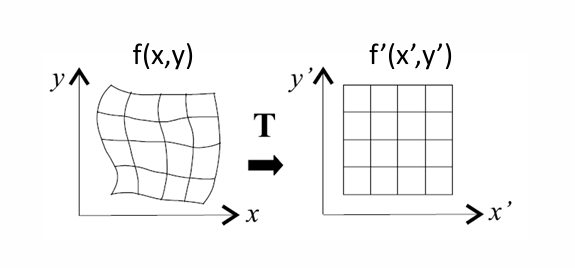
\includegraphics[width=0.5\textwidth]{img/geom_tran.png}
 \caption{Geometrické transformace}
 \end{figure}

 Při výpočtu geometrické transformace dochází k: 1) Transformacisouřadnic, mapování (x,y) na (x',y'). 2 ) k interpolací jasových hodnot - určení nové jasové hodnoty v místě
 mimo ortogonální rastr.

 Geometrické transformace převádí int na real, ale stále výsledek musí být v pravidelné vzorkovací mřížce.
 Následkem je vznik děr a nejednoznačnost - na jednu pozice se mapuje více pixelů.

Obecně geometrická transformace neexistuje, pokaždé se jedná o jejich aproximací

\subsection{Aproximace}

\[
x' = \sum_{r=0}^{n} \sum_{k=0}^{\,n-r} a_{rk} \cdot x^{r} \cdot y^{k}
\]
\[
y' = \sum_{r=0}^{n} \sum_{k=0}^{\,n-r} b_{rk} \cdot x^{r} \cdot y^{k}
\]
n - je voleno podle míry zkreslení , pokud v nekorigovaném obrazu nedochází k rychlým změnám souřadnic -> n <= 3
\textbf{bilineární transformace: }
(n=2)
$x' = a_0 +a_1*x + a_2*y + a3*x*y$ pokracuje: $+a_4*x^2+a_5*y^2$
$y' = b_0 +b_1*x + b_2*y + b3*x*y$ pokracuje: $+b_4*x^2+b_5*y^2$

\textbf{Affinní transformace: }
(n=1)
$x' = a_0 +a_1*x + a_2*y$ 
$y' = b_0 +b_1*x + b_2*y$

Operace proveditelné zapomocí afinního tvaru:
\begin{itemize}
    \item posunutí : členy a0 a b0
    \item rotace : členy a1,a2 a b1 a b2 (sin/cos)
    \item měřítko : členy a1 a b2
    \item zkosení : členy a2 a b1
\end{itemize}
\subsection{Homogenní souřadnice}
– reprezentace bodu v prostoru o jednu dimenzi vyšším, než odpovídá skutečné dimenzi bodu

\[
P = 
\begin{bmatrix}
x \\ y
\end{bmatrix}
\quad \Rightarrow \quad
P_H =
\begin{bmatrix}
\lambda x \\ \lambda y \\ \lambda
\end{bmatrix},
\qquad \lambda \neq 0
\]

Affinní transformace v homogenních souřadnicích:

\[
x' = a_0 + a_1 x + a_2 y
\]
\[
y' = b_0 + b_1 x + b_2 y
\]
\[
\begin{bmatrix}
x' \\
y' \\
1
\end{bmatrix}
=
\begin{bmatrix}
a_1 & a_2 & a_0 \\
b_1 & b_2 & b_0 \\
0   & 0   & 1
\end{bmatrix}
\cdot
\begin{bmatrix}
x \\
y \\
1
\end{bmatrix}
\]

\subsection{Interpolace souřadnic}
Výstupní obraz musí mít stejně jako vstupní pevnou rastrovou mřížku. Dochází k neceločíselným souřadnicím, tím pádem nejde přesně určit jasovou hodnotu a proto je nutné interpolovat
Metody interpolace:
\begin{itemize}
    \item nejbližší soused
    \item statistika - N nejbližších sousedů (často prostý průměr 4 nejbližších sousedů)
    \item lineární / bilineární/trilineární interpolace (tj. linearizace 1D/2D/3D)
    \item kubická/bikubická/trikubická interpolace (tj. polynomizace signálu v 1D/2D/3D)
\end{itemize}
Peostě popis jak fungujou konkrétní interpolace..
\subsection{Korekce zkreslení}


\text{aproximujeme analytickou funkcí odpovídající předpokládanému zkreslení.}

\subsubsection{Radiální zkreslení (soudek, poduška)}
r = \text{radiální vzdálenost bodu } (x, y) \text{ od středu obrazu (nebo jiného vztažného bodu).}
\[
x' = x \cdot \left( 1 + \kappa_1 r^2 + \kappa_2 r^4 + \kappa_3 r^6 \right)
\]
\[
y' = y \cdot \left( 1 + \kappa_1 r^2 + \kappa_2 r^4 + \kappa_3 r^6 \right)
\]
\subsubsection*{Tangenciální zkreslení (perspektiva)}
\[
x' = x + 2\rho_1 y + \rho_2 (r^2 + 2x^2)
\]
\[
y' = y + 2\rho_2 x + \rho_1 (r^2 + 2y^2)
\]


\subsection{Rotace}

\subsubsection*{Otočení obrazu o 90°, 180° a 270°}
\begin{itemize}
    \item záměna řádků a sloupců
    \item nedochází ke zkreslením, tj. $\mathrm{rot}(90^\circ) \neq \mathrm{rot}(\mathrm{rot}(45^\circ))$
\end{itemize}

\subsubsection*{Otočení obrazu o libovolný úhel $\alpha$ – definice}
\[
x' = a_0 + a_1 x + a_2 y
\]
\[
y' = b_0 + b_1 x + b_2 y
\]
kde 
\[
\{a_0, b_0\} \rightarrow 0, \qquad 
\{a_1, a_2, b_1, b_2\} \rightarrow \{\sin, \cos\}
\]
\[
\Downarrow
\]
\[
\begin{bmatrix}
x' \\
y' \\
1
\end{bmatrix}
=
\begin{bmatrix}
\cos \alpha & -\sin \alpha & 0 \\
\sin \alpha & \cos \alpha & 0 \\
0 & 0 & 1
\end{bmatrix}
\cdot
\begin{bmatrix}
x \\
y \\
1
\end{bmatrix}
\]



\section{Morfologické operace a integrální transformace (využití FT pro zpracování vícerozměrných signálů - vzorce,
vlastnosti, výhody a nevýhody, typy a tvorba filtrů, korelace a autokorelace).}